\documentclass[UTF8]{article}
    \title{梯度法求解时间最优量子比特重置（$\boldsymbol{\sigma_x}$）\\\large 最优控制问题直接法求解工具箱}
    \author{黄泓博}
    \date{\today}

\usepackage[dvipsnames, svgnames, x11names]{xcolor}
\usepackage{ctex}
\usepackage{mathdesign}
\usepackage{mathtools}
\usepackage{physics}
\usepackage{mhchem}
\usepackage{chemfig}
\usepackage{color}
\usepackage{mathrsfs}
\usepackage{siunitx}
    \sisetup{
        range-phrase=\sim,
        range-units=single,
        list-separator={, },
        list-final-separator={\text{和}},
        list-pair-separator={\text{和}},
        list-units=single,
    }
\usepackage{amsmath}
    \numberwithin{equation}{section}
\usepackage{amsthm}
\usepackage{amssymb}
\usepackage{geometry}
    %\geometry{left=3.18cm,right=3.18cm,top=2.54cm,bottom=2.54cm}
\usepackage{picture}
    \usepackage{subfigure}
\usepackage{array}
    \usepackage{booktabs}
    \usepackage{colortbl}
\usepackage{tikz}
    \usetikzlibrary{positioning, arrows.meta}
\usepackage{listings}
    \lstset{language=Matlab}
\usepackage[framed,numbered,autolinebreaks,useliterate]{mcode}
\usepackage{textcomp}
\usepackage{upgreek}
\usepackage{multirow}
\usepackage{cite}
\usepackage{hyperref}
    \hypersetup{
        colorlinks = true,
        linkcolor = blue,
        filecolor = blue,
        urlcolor = blue,
        citecolor = blue,
    }
    \usepackage{hycolor}
\usepackage{ulem}
\usepackage{booktabs}

\allowdisplaybreaks[4]

\newcommand{\mi}{\mathrm{i}}
\newcommand{\me}{\mathrm{e}}
\newcommand{\expe}{\mathrm{E}}
\newcommand{\eqty}{\left<\right>}
\newcommand{\ad}{\mathrm{ad}}
\newcommand{\defeq}{\overset{\mathrm{def}}{=}}

\begin{document}
    \maketitle
    \begin{abstract}
        现成封装的商用最优控制求解器（如基于 CasADi/IPOPT 的直接法）通常不会输出迭代的中间过程，这使得无法直观地调试收敛过程。本工作面向\textbf{含$\sigma_x$驱动的量子比特重置}这一时间最优控制问题，从零编写了一个\textbf{直接法梯度求解器}，它以输出每次迭代的状态、协态、控制与成本为设计目标，从而能够定位并解决收敛过程中的问题。工具箱将具体的\textbf{最优控制问题}与\textbf{求解算法}解耦：只需按抽象接口提供一个问题，即可用同一套算法求解。
        \par
        本文档首先介绍梯度法的理论（庞特里亚金极值原理）、有约束情况的两种处理（惩罚函数与投影梯度法）、历史累计的方向优化（Adagrad、RMSprop、经典动量、Nesterov、Adam）以及步长搜索准则；随后给出要解决的量子比特重置控制论问题；最后介绍为解决\textbf{梯度消失}与\textbf{初值敏感}问题而引入的正则化与同伦延拓（数值延拓 / prolong），以及整个工具箱的程序结构和可替换问题的方法。
    \end{abstract}

    \section{待求最优控制问题的抽象与工具箱结构}
        本工具箱的核心思想是：把"待求的最优控制问题"抽象成一个接口，把"求解算法"实现为通用的可复用组件。只要一个具体问题满足该接口，就可以用同一套梯度求解器去解它。
        \par
        \textbf{抽象接口（\texttt{ocp.AbstractOCP}）}：一个最优控制问题只需提供以下内容——
        \begin{itemize}
            \item 状态维数、控制维数、总时长 $\tau$；
            \item 时间格点 $\vb*{t}_\mathrm{grid}$ 与初态 $\vb*{x}_0$；
            \item 初始控制的猜测 $\vb*{u}^{\pqty{0}}\pqty{t}$；
            \item 目标泛函及其对控制的（离散）梯度 $\pqty{J,\pdv{J}{\vb*{u}}}$；
            \item 控制的可行域（长方体约束）及其投影。
        \end{itemize}
        求解器\textbf{只}依赖这些内容，完全不关心问题的物理细节。
        \par
        \textbf{具体问题}：\texttt{ocp.QubitReset}（本工作求解的含$\sigma_x$量子比特重置问题）与 \texttt{ocp.ControlExample}（一个独立的、可解析求解的示例问题，见第\ref{sec:control}节末尾）。二者实现同一接口，故同一求解器可直接替换使用。
        \par
        \textbf{求解算法（\texttt{solver.GradientSolver}）}：在下文各节中描述，集成了投影梯度、历史累计方向优化与多种步长搜索准则。
        \par
        \textbf{同伦延拓外壳（\texttt{continuation.HomotopyContinuation}）}：一个与具体问题无关的延拓层，用于处理梯度消失与初值敏感问题，见第\ref{sec:prolong}节。
        \par
        因此，要解决\textbf{另一个}最优控制问题，只需实现 \texttt{ocp.AbstractOCP} 接口，不需要修改任何求解算法。

    \section{梯度法}\footnote{本小节内容参考\textit{最优化与最优控制（第二版），赫孝良，葛照强，西安交通大学出版社，2015}.}
        在打靶法和配点法之前，先介绍梯度法，该方法既不离散化控制，也不离散化状态，而是直接通过梯度下降法迭代整个过程中的控制.
        \subsection{无约束的情况}
            将最优控制问题写成哈密顿形式
            \begin{align}
                L_\text{aug}=&L+\vb*{\lambda}^\text{T}\pqty{\dot{\vb*{x}}-\vb*{f}}\\
                H=&\vb*{\lambda}^\text{T}\dot{\vb*{x}}-L_\text{aug}
                =&\vb*{\lambda}^\text{T}\vb*{f}-L
            \end{align}
            于是欧拉-拉格朗日方程变为协态方程（哈密顿正则方程之二）
            \begin{align}
                \dot{\vb*{\lambda}}=-\pdv{H}{\vb*{x}}
            \end{align}
            在上式和运动方程（哈密顿正则方程之一）的约束下，求解哈密顿量$H$的极值
            \begin{align}
                \pdv{H}{\vb*{u}}=0
            \end{align}
            进一步地，庞特里亚金最优化原理还告诉我们，此时哈密顿应为常数.
            \par
            在写出最优控制问题的哈密顿量后，梯度法的主要步骤可以写作
            \begin{enumerate}
                \item 猜测初始控制$\vb*{u}^\pqty{k=0}\pqty{t}$.
                \item 将$\vb*{u}^\pqty{k}\pqty{t}$带入哈密顿正则方程，积分得到$\vb*{x}^\pqty{k}\pqty{t}$和$\vb*{\lambda}^\pqty{k}\pqty{t}$.
                \item 用此时的$\vb*{u}^\pqty{k}\pqty{t},\vb*{x}^\pqty{k}\pqty{t}$和$\vb*{\lambda}^\pqty{k}\pqty{t}$计算此时的梯度$\pdv{H}{\vb*{u}}^\pqty{k}$.
                \item 利用梯度迭代控制$\vb*{u}^\pqty{k+1}\pqty{t}=\vb*{u}^\pqty{k}\pqty{t}+h^\pqty{k}\pdv{H}{\vb*{u}}^\pqty{k}$，其中$h^\pqty{k}$为步长.
                \item 计算梯度的大小$\abs{\pdv{H}{\vb*{u}}^\pqty{k}}$，判断其是否小于设定精度$\epsilon$.若否，则返回第二步.
                \item 符合条件，终止.
            \end{enumerate}
            \par
            {\color{blue}
                \textbf{例1}：控制论问题
                \begin{itemize}
                    \item \textbf{运动方程：}$\dot{x}=-x^2+u$.
                    \item \textbf{边界约束：}$x\pqty{0}=10$，$t=1$末态时刻为自由边界.
                    \item \textbf{目标函数：}$J=\int_{0}^{1}\frac{1}{2}\pqty{x^2+u^2}\dd{t}$.
                \end{itemize}
                \par
                \textbf{解}：首先写出哈密顿量
                \begin{align}
                    L=&\frac{1}{2}\pqty{x^2+u^2}\\
                    L_\text{aug}=&\frac{1}{2}\pqty{x^2+u^2}+\lambda\pqty{\dot{x}+x^2-u}\\
                    H=&\lambda\pqty{-x^2+u}-\frac{1}{2}\pqty{x^2+u^2}
                \end{align}
                和协态方程
                \begin{align}
                    \dot{\lambda}=-\pdv{H}{x}=2x\lambda+x
                \end{align}
                $t=1$时刻为自由边界，给出自然边界条件$\eval{\pdv{L_\text{aug}}{\dot{x}}}_{t=t_f}=0$给出
                \begin{align}
                    \lambda\pqty{1}=0
                \end{align}
                求梯度得
                \begin{align}
                    \pdv{H}{u}=\lambda-u
                \end{align}
                \begin{figure}[htb]
                    \centering
                    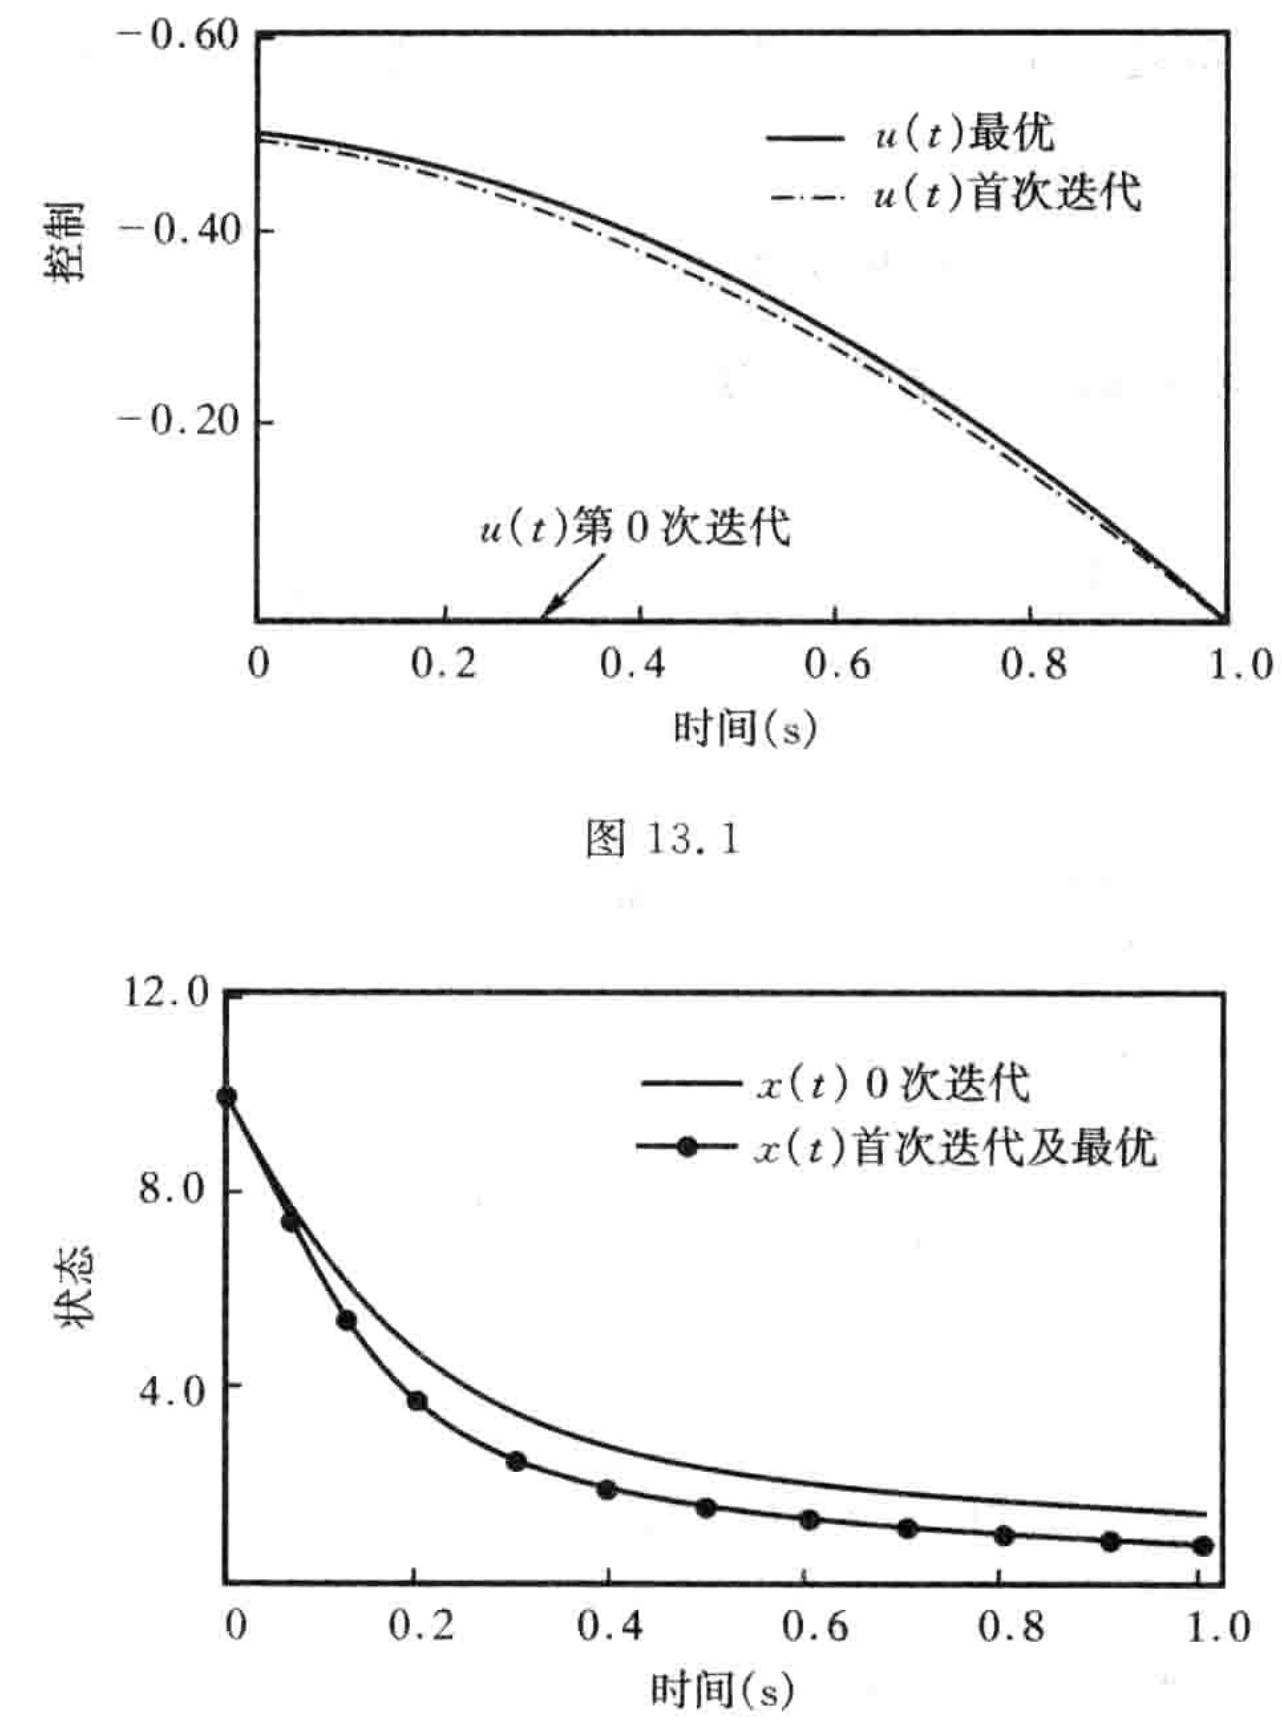
\includegraphics[width=0.5\textwidth]{例12.1.jpg}
                    \caption{例1首次迭代得到的结果}
                \end{figure}
                迭代求解.事实上，因为该问题较为简单，首次迭代的效果就已经很好了.
                \qed
            }
            \par
            该例1对应工具箱中的 \texttt{ocp.ControlExample} 问题。它没有末态成本，而是一条运行成本积分，因此哈密顿量中的运行项$\pqty{-L}$不可忽略。用同一求解器可求解该问题，以验证所谓"可替换问题"的抽象性.
            \par
            梯度法可以拓展到高阶情况，即考虑$H$的高阶导数.除了提高阶数之外，还有共轭梯度法、变尺度方法等推广自静态最优的方法.此略.
            \par
            梯度法的缺点也是明显的：它仍然需要利用哈密顿量$H$及其梯度$\pdv{H}{\vb*{u}}$的解析表达式；另一方面，其收敛效果受步长选取的影响较大，在后文中会提供一些步长搜索准则来缓解这个缺点.

    \section{有约束的情况：惩罚函数}
        将边界约束和路径约束转化为突破约束的惩罚函数，对目标函数进行增广
        \begin{align}
            J_\text{aug}=&K+\int_{t_0}^{t_f}L\dd{t}
            +\vb*{\phi}^\text{T}\vb*{G}\vb*{\phi}+\int_{t_0}^{t_f}\sum_{i}g_i\abs{C_i}^P\Theta\pqty{C_i}\dd{t}
        \end{align}
        其中$\Theta\pqty{x}$为阶跃函数.$\vb*{G}$为一正（负）定对称矩阵，$\vb*{g}$为一全正（负）向量，当它们趋近于$\pm\infty$时，求解增广目标函数最小（大）值的问题将等价于在边界约束和路径约束下求解原目标函数的最小（大）值.在实际数值计算中，调节$\vb*{G}$和$\vb*{g}$究竟取多大取决于我们的精度要求，一般取$P=2$.
        \par
        {\color{blue}
            \textbf{例2}：控制论问题
            \begin{itemize}
                \item \textbf{运动方程：}$\dot{x}=u$.
                \item \textbf{边界约束：}$x\pqty{0}=1,x\pqty{1}=0$.
                \item \textbf{目标函数：}$J=\int_{0}^{1}u^2\dd{t}$.
            \end{itemize}
            \par
            \textbf{解}：将末态改为自由边界，约束写进增广目标函数中
            \begin{align}
                J_\text{aug}=Gx\pqty{1}^2+\int_{0}^{1}u^2\dd{t}
            \end{align}
            哈密顿量及正则方程
            \begin{align}
                H=&u^2+\lambda u\\
                \dot{\lambda}=&-\pdv{H}{x}=0
            \end{align}
            $t=1$时刻自由边界的自然边界条件$\lambda\pqty{1}=2Gx\pqty{1}$，解得$x\pqty{t}=1-\frac{G}{1+G}t$.当$G\to\infty$时，$x\pqty{1}\to0$，最优控制$u\pqty{t}=-1$.
            \qed
        }
        \par
        惩罚函数法在数值上往往\textbf{不稳定}：当惩罚因子$g$较大时，目标函数会变得刚性，容易导致震荡甚至发散。因此本工具箱默认采用下一节更稳定的\textbf{投影梯度法}来纳入路径约束。

    \section{投影梯度下降法}
        投影梯度下降法把约束的处理从"惩罚"改为"投影".其迭代为
        \begin{align}
            \vb*{u}^\pqty{k+1}\pqty{t}=\vb*{Proj}\pqty{\vb*{u}^\pqty{k}\pqty{t}+h^\pqty{k}\pdv{H}{\vb*{u}}^\pqty{k}}
        \end{align}
        其中$\vb*{Proj}$为向控制的可行域（对量子比特重置问题是一个长方体$\lambda_x\in\bqty{0,\lambda_x^\pqty{m}}$，$\lambda_z\in\bqty{0,\lambda_z^\pqty{m}}$）的投影.数学上可以证明，投影操作不影响收敛性；对于可分离的长方体约束，它甚至也不怎么额外消耗性能.
        \par
        需要注意"定义在边界处的梯度"：当某个控制分量已经到达其上（下）界，且梯度继续把它往外推时，该分量该方向的"有效梯度"应为零。这相当于把控制约束的互补松紧条件（KKT 活动集）并入梯度。本工具箱在投影梯度的基础上，通过活动集检测（\texttt{kktActiveSet} 选项）实现这一点.

    \section{历史累计的方向优化}
        在上一节的梯度下降法中，算法迭代的方向仅由梯度决定$\vb*{d}^\pqty{k}=\pdv{H}{\vb*{u}}^\pqty{k}$.这可能会遇到一些困难，如图\ref{FigSaddle}鞍点跨越就是其中的一个.
        \begin{figure}[htb]
            \centering
            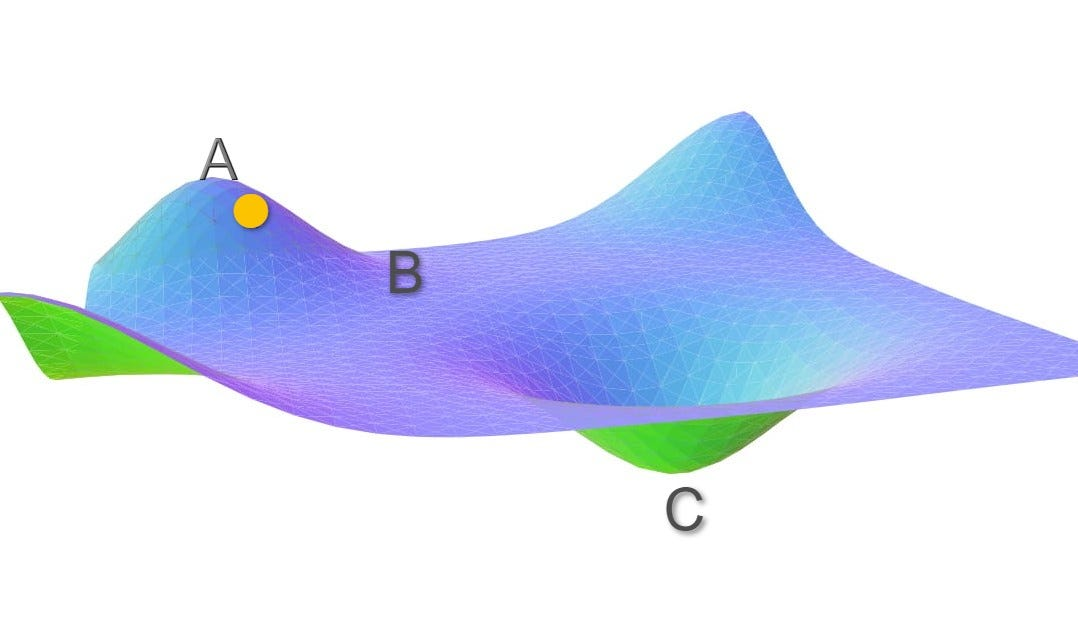
\includegraphics[width=0.6\textwidth]{鞍点.jpeg}
            \caption{鞍点跨越的示意图.当程序从初值A点处开始优化，最开始梯度指引的下降方向很明确，但是当下降到B点后，就进入了所谓的高原区（Plateau Region），需要进行鞍点跨越（Saddle Point Traversal）才能进一步下降.}
            \label{FigSaddle}
        \end{figure}
        \par
        累计梯度的历史来改进优化的方向会是一件有所帮助的事情.下面介绍工具箱实现的各种方向优化算法。对量子比特重置问题，梯度法是收敛较慢的，且倾向于在高原区停滞；采用这些"历史累计的方向"能显著改善跨越鞍点和高原区的能力。
        \label{sec:dir}
        \par
        \textbf{记号约定}：设$k$为迭代次数，$\vb*{g}^\pqty{k}\defeq\pdv{H}{\vb*{u}}^\pqty{k}$为当前步的梯度方向（工具箱内部以"目标泛函的梯度"$\pdv{J}{\vb*{u}}$存储，二者只差一个符号，不影响方向），$\vb*{d}^\pqty{k}$为实际采用的更新方向，$\vb*{u}^\pqty{k+1}=\vb*{u}^\pqty{k}+h^\pqty{k}\vb*{d}^\pqty{k}$. 分量运算均为逐元素进行.
        \subsection{自适应梯度（Adaptive Gradient, Adagrad）}
            Adagrad维护历史梯度平方的累计
            \begin{align}
                \vb*{G}^\pqty{k}=\vb*{G}^\pqty{k-1}+\pqty{\vb*{g}^\pqty{k}}^2
            \end{align}
            并用其平方根对当前梯度缩放，从而自动减小更新步长，适应不同参数的稀疏性：
            \begin{align}
                \vb*{d}^\pqty{k}=-\frac{\vb*{g}^\pqty{k}}{\sqrt{\vb*{G}^\pqty{k}}+\epsilon}
            \end{align}
            其中$\epsilon$为防止除零的小量.Adagrad适合稀疏梯度问题，但累计项会不断增大，导致步长单调递减，可能退化失效.
        \subsection{均方根传播（Root Mean Square Propagation, RMSprop）}
            RMSprop通过对历史平方梯度采用指数加权移动平均（EMA），限制累计项增长：
            \begin{align}
                \vb*{E}^\pqty{k}=\beta_2\vb*{E}^\pqty{k-1}+\pqty{1-\beta_2}\pqty{\vb*{g}^\pqty{k}}^2
            \end{align}
            \begin{align}
                \vb*{d}^\pqty{k}=-\frac{\vb*{g}^\pqty{k}}{\sqrt{\vb*{E}^\pqty{k}}+\epsilon}
            \end{align}
            其中$\beta_2$为二阶矩衰减系数.它保留了Adagrad的自适应能力，又避免了过度衰减.
        \subsection{经典动量（Classical Momentum, CM）}
            Polyak重球法引入动量：
            \begin{align}
                \vb*{d}^\pqty{k}=\beta_1\vb*{d}^\pqty{k-1}+\pqty{1-\beta_1}\vb*{g}^\pqty{k}
            \end{align}
            其中$\beta_1$为一阶矩（动量）衰减系数.动量项帮助克服鞍点和高原区，减少震荡.
        \subsection{Nesterov加速梯度（Nesterov Accelerated Gradient, NAG）}
            NAG在计算梯度前先用动量"预看"一步：
            \begin{align}
                \vb*{d}^\pqty{k}=\beta_1\vb*{d}^\pqty{k-1}+\pqty{1-\beta_1}\eval{\pdv{H}{\vb*{u}}}_{\vb*{u}^\pqty{k}+\beta_1\vb*{d}^\pqty{k-1}}
            \end{align}
            预看点可能已越过梯度为零的平坦区，能提供更有用的方向信息（例如指向鞍点的下坡方向），在鞍点和高原区表现更优.
        \subsection{自适应矩估计（Adaptive Moment Estimation, Adam）}
            Adam同时维护梯度的一阶矩（动量）与二阶矩（历史）的EMA，并进行偏差校正：
            \begin{align}
                \vb*{v}^\pqty{k}&=\beta_1\vb*{v}^\pqty{k-1}+\pqty{1-\beta_1}\vb*{g}^\pqty{k}\\
                \vb*{m}^\pqty{k}&=\beta_2\vb*{m}^\pqty{k-1}+\pqty{1-\beta_2}\pqty{\vb*{g}^\pqty{k}}^2
            \end{align}
            \begin{align}
                \hat{\vb*{v}}^\pqty{k}=&\frac{\vb*{v}^\pqty{k}}{1-\beta_1^k} &
                \hat{\vb*{m}}^\pqty{k}=&\frac{\vb*{m}^\pqty{k}}{1-\beta_2^k}
            \end{align}
            \begin{align}
                \vb*{d}^\pqty{k}=-\frac{\hat{\vb*{v}}^\pqty{k}}{\sqrt{\hat{\vb*{m}}^\pqty{k}}+\epsilon}
            \end{align}
            Adam兼具自适应性与动量的特点.
        \par
        \textbf{与线搜索配合的注意点}：动量类方法的$\vb*{d}^\pqty{k}$并不一定是下降方向。工具箱在与线搜索配合时，会先判断当前方向是否下降（即$\pqty{\pdv{J}{\vb*{u}}}^{T}\vb*{d}^\pqty{k}<0$），若非下降方向则本轮不更新.这正是动量方法所需的额外程序设计（见 \texttt{GradientSolver} 源码）.

    \section{步长搜索准则}\footnote{本小节内容参考\textit{最优化理论与方法，袁亚湘，孙文瑜，科学出版社，1997}.}
        步长的选取对梯度法的收敛很重要.这不仅体现在变步长方法可以加快收敛的速度，不合适的步长选取甚至会导致迭代在最优解附近反复横跳、难以收敛的情况.一般只采用一些非精确搜索的准则即可.
        \label{sec:step}
        \begin{figure}[htb]
            \centering
            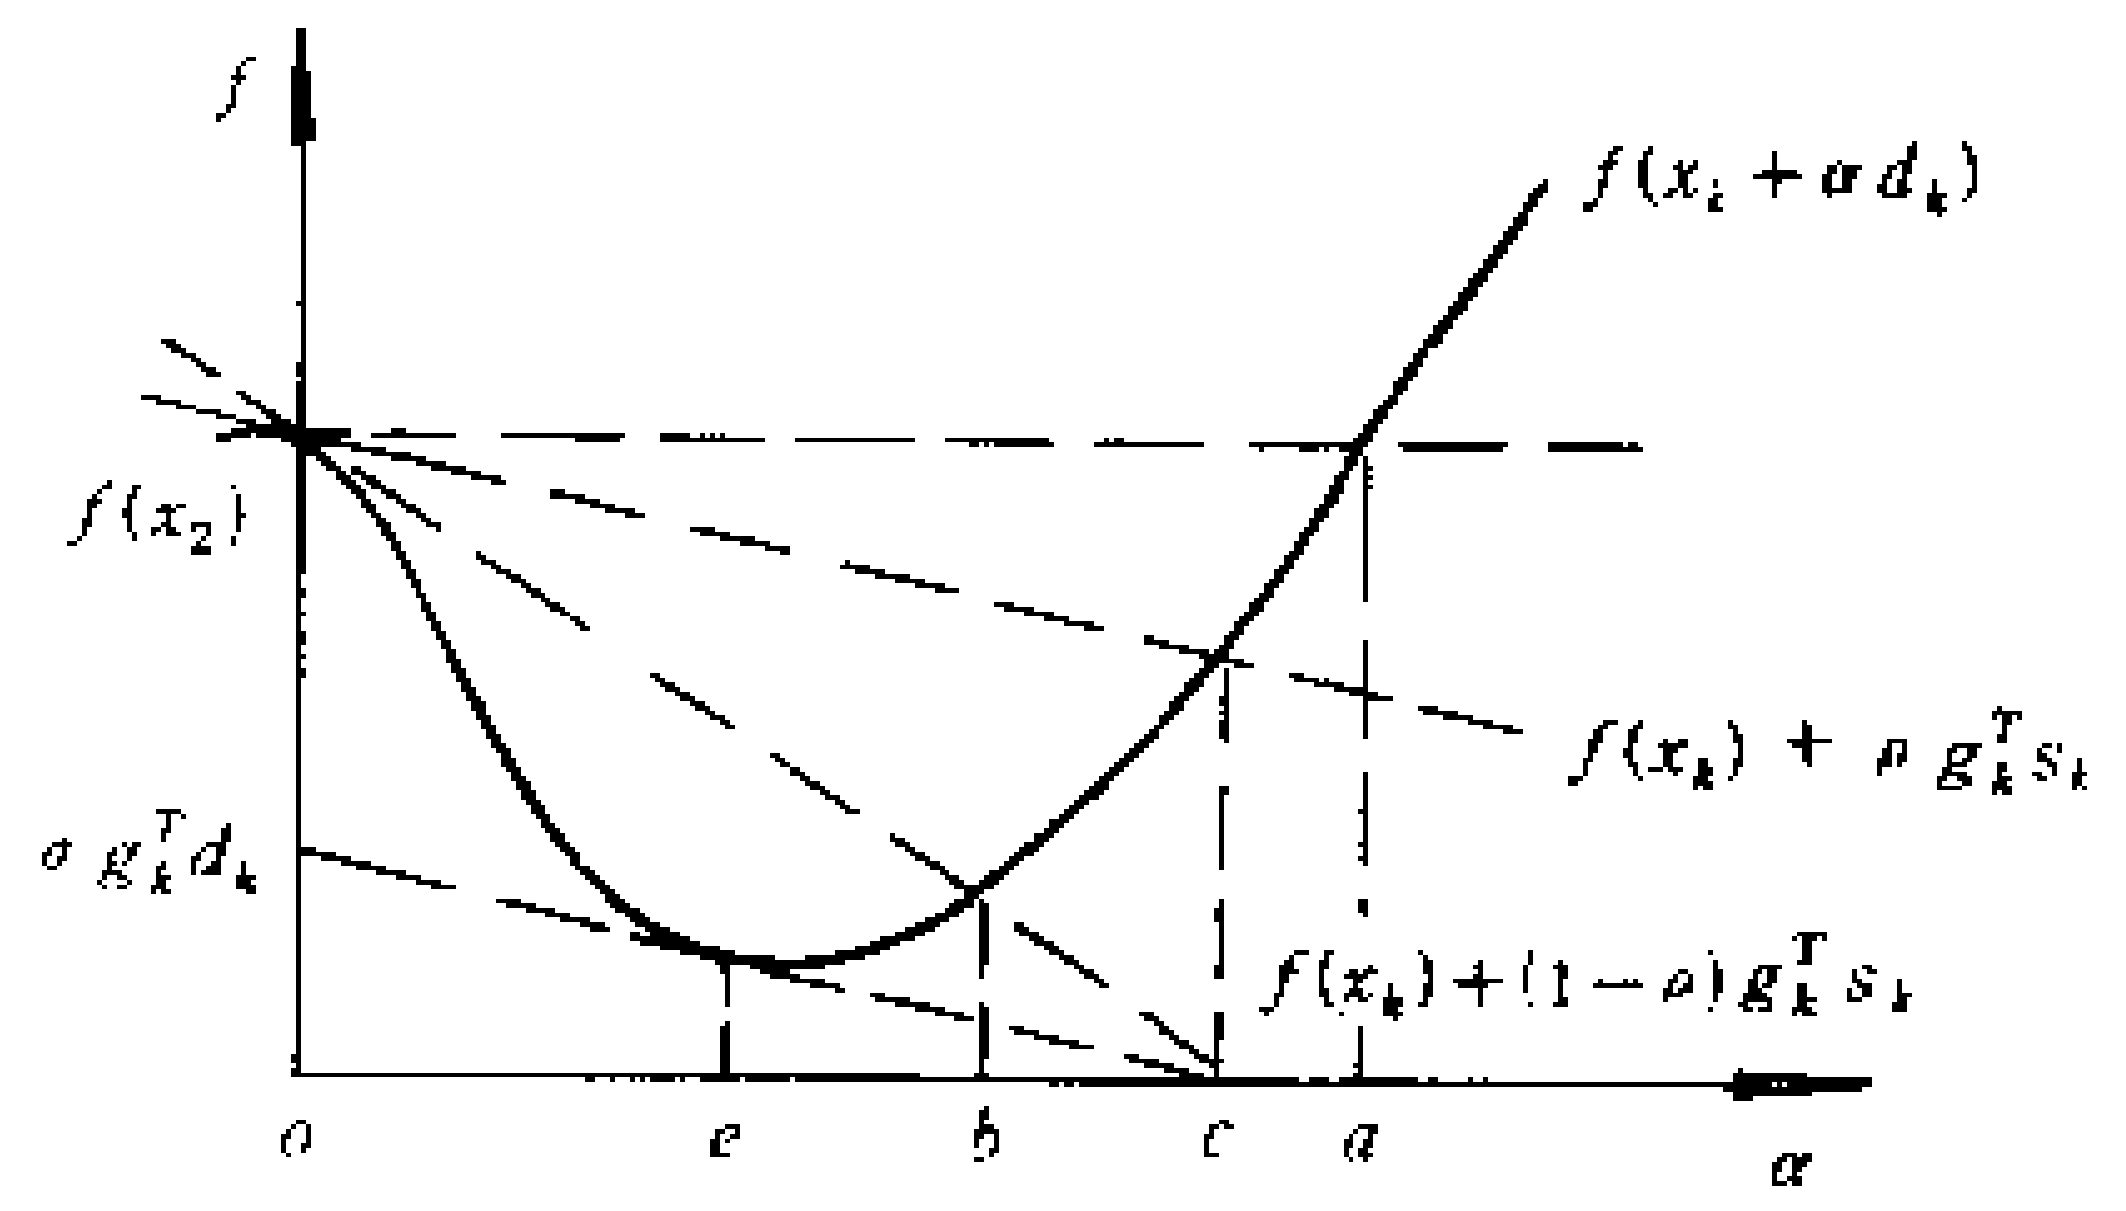
\includegraphics[width=0.6\textwidth]{准则.jpg}
            \caption{准则的示意图.区间$\pqty{0,a}$为让函数值下降的区间，即梯度下降法能正常工作的区间.区间$\pqty{0,c}$为简单准则的可接受区间.区间$\pqty{b,c}$为Armijo-Goldstein准则的可接受区间，极值点有可能被排除在其外.区间$\pqty{e,c}$为Wolfe-Powell准则的可接受区间.}
        \end{figure}
        \par
        单纯形准则要求步长$h^\pqty{k}$不应该太靠近区间的右边界$a^\pqty{k}$：
        \begin{align}
            f\pqty{x^\pqty{k}+s^\pqty{k}}\leq f\pqty{x^\pqty{k}}+\rho f'\pqty{x^\pqty{k}}s^\pqty{k}
        \end{align}
        其中$\rho\in\pqty{0,\frac12}$.这被称为后退方法（backtracking），通常简单地把步长减半即可.
        \par
        \textbf{Armijo-Goldstein准则}在简单准则基础上，为防止步长太小给出额外条件（不靠近左边界）：
        \begin{align}
            f\pqty{x^\pqty{k}+s^\pqty{k}}\geq f\pqty{x^\pqty{k}}+\pqty{1-\rho}f'\pqty{x^\pqty{k}}s^\pqty{k}
        \end{align}
        \par
        \textbf{Wolfe-Powell准则}给出更简单的左边界条件：
        \begin{align}
            f'\pqty{x^\pqty{k}+s^\pqty{k}}d^\pqty{k}\geq\sigma f'\pqty{x^\pqty{k}}d^\pqty{k}
        \end{align}
        其中$\sigma\in\pqty{\rho,1}$.对于非精确搜索一般取$\rho=0.1,\sigma=0.4$.本工具箱的 \texttt{solver.LineSearch} 实现了这三种准则，并支持二分法插值.

    \section{要解决的控制论问题}\label{sec:control}
        要解决的控制论问题为给定擦除时间，找到擦除精度最高的擦除路径.
        \begin{itemize}
            \item \textbf{状态与控制：}系统的状态$\vb*{p}=\pqty{p_e,p_r,p_i}$，控制为$\pqty{\lambda_x,\lambda_z}$.
            \item \textbf{运动方程：}$\dot{\vb*{p}}=\vb*{P}\vb*{p}+\vb*{p}_0$.
            \item \textbf{边界约束：}$\vb*{p}\pqty{0}=\pqty{0.5,0,0}$；$t=\tau$末态时刻为自由边界，有自然边界条件见下文.
            \item \textbf{路径约束：}控制的路径约束$\lambda_x\in\bqty{0,\lambda_x^\pqty{m}},\lambda_z\in\bqty{0,\lambda_z^\pqty{m}}.$
            \item \textbf{目标函数：}$J=\abs{\vb*{p}\pqty{\tau}}$.
        \end{itemize}
        其中
        \begin{align}
            &\vb*{P}=\pmqty{
                -\gamma\pqty{4\Gamma_z\sin^2\theta+\pqty{\Gamma_++\Gamma_-}\pqty{1+\cos^2\theta}}&\gamma\pqty{4\Gamma_z-\Gamma_+-\Gamma_-}\cos\theta\sin\theta&-2\Lambda\sin\theta\\
                \gamma\pqty{4\Gamma_z-\Gamma_+-\Gamma_-}\cos\theta\sin\theta&-\gamma\pqty{4\Gamma_z\cos^2\theta+\pqty{\Gamma_++\Gamma_-}\pqty{1+\sin^2\theta}}&2\Lambda\cos\theta\\
                2\Lambda\sin\theta&-2\Lambda\cos\theta&-\gamma\pqty{4\Gamma_z+\Gamma_++\Gamma_-}
            }
        \end{align}
        \begin{align}
            \vb*{p}_0=&\pmqty{
                \gamma\pqty{2\Gamma_z\sin^2\theta+\frac{1}{2}\pqty{\Gamma_+\pqty{1-\cos\theta}^2+\Gamma_-\pqty{1+\cos\theta}^2}}\\
                -\gamma\pqty{2\Gamma_z\cos\theta\sin\theta-\frac{1}{2}\pqty{\Gamma_+\sin\theta\pqty{\cos\theta-2}+\Gamma_-\sin\theta\pqty{\cos\theta+2}}}\\
                -\Lambda\sin\theta
            }
        \end{align}
        \begin{align}
            \Gamma_z\pqty{t}=&\pi\sin^2\theta\pqty{t}\\
            \Gamma_\pm\pqty{t}=&\cos^2\theta\pqty{t}\frac{1}{2}J\pqty{2\Lambda\pqty{t}}\pqty{\coth\pqty{\Lambda\pqty{t}}\pm 1}\\
            J\pqty{\omega}=&\pi\omega\frac{\omega_c^2}{\omega_c^2+\omega^2}
        \end{align}
        其中
        \begin{align}
            \theta\pqty{t}=\arctan\frac{\lambda_x}{\lambda_z}, \qquad \Lambda\pqty{t}=\sqrt{\lambda_x^2+\lambda_z^2}
        \end{align}
        密度矩阵的正定性要求会给出状态的路径约束，主方程会保证其在物理上自然满足，故不特意写出.
        \par
        哈密顿量
        \begin{align}
            H=\vb*{\mu}^\text{T}\pqty{\vb*{P}\vb*{p}+\vb*{p}_0}-L
        \end{align}
        正则方程
        \begin{align}
            \dot{\vb*{p}}=&\vb*{P}\vb*{p}+\vb*{p}_0\\
            \dot{\vb*{\mu}}=&-\vb*{P}^\text{T}\vb*{\mu}
        \end{align}
        当$L=0$（纯末态成本）时，自由边界的自然边界条件给出
        \begin{align}
            \vb*{\mu}\pqty{\tau}+\frac{\vb*{p}\pqty{\tau}}{\abs{\vb*{p}\pqty{\tau}}}=0
            \qquad\Longrightarrow\qquad
            \vb*{\mu}\pqty{\tau}=-\frac{\vb*{p}\pqty{\tau}}{\abs{\vb*{p}\pqty{\tau}}}
        \end{align}
        梯度
        \begin{align}
            \pdv{H}{\pqty{\lambda_x,\lambda_z}}=\vb*{\mu}^\text{T}\pqty{\pdv{\vb*{P}}{\pqty{\lambda_x,\lambda_z}}\vb*{p}+\pdv{\vb*{p}_0}{\pqty{\lambda_x,\lambda_z}}}-\pdv{L}{\pqty{\lambda_x,\lambda_z}}
        \end{align}
        其中
        \begin{align}
            \pdv{\pqty{\theta,\Lambda}}{\pqty{\lambda_x,\lambda_z}}=\pmqty{\frac{\lambda_z}{\Lambda^2}&-\frac{\lambda_x}{\Lambda^2}\\\frac{\lambda_x}{\Lambda}&\frac{\lambda_z}{\Lambda}}
        \end{align}
        \par
        \textbf{梯度消失问题}：由于系统的动力学是\textbf{耗散}的，而成本是\textbf{末端函数}$\abs{\vb*{p}\pqty{\tau}}$，当擦除时间$\tau$较长时，末端对初态（进而对初始控制）的敏感性会下降，导致梯度$\pdv{H}{\vb*{u}}$在迭代初期趋于零，梯度法难以启动。这正是引入下一节正则化与同伦延拓的动机.
        \par
        \textbf{可替换性示例}：\texttt{ocp.ControlExample}（本节例1）实现了同一接口，但它是一个标量状态/控制、带运行成本的问题。同一个 \texttt{solver.GradientSolver} 无需任何修改即可求解它，这体现了"把待求问题抽象为可替换工具"的设计.

    \section{正则化与同伦延拓}\label{sec:prolong}
        为解决梯度消失与初值敏感问题，本工具箱提供\textbf{同伦延拓}（数值延拓 / prolongation）机制：把原问题嵌入到一族参数化的问题中，从一个\textbf{容易求解}的子问题出发，逐步把参数推进到原问题的参数，每一步以上一步的最优解作为初始猜测（warm start）.
        \par
        在量子比特重置问题中，工具箱支持两种延拓族（由 \texttt{QubitReset.homotopyName} 选择）：
        \begin{enumerate}
            \item \textbf{时域延拓（$\texttt{homotopyName}=\texttt{'tau'}$）}：从较短的擦除时间$\tau_0$逐步增大到目标$\tau$。短时间时末端对初态仍敏感，梯度不消失，先解出再外推，从而绕过初始位置梯度消失的问题。
            \item \textbf{成本权重延拓（$\texttt{homotopyName}=\texttt{'kappa'}$）}：为成本添加一个正则化运行项，并从$\kappa=0$逐步增大到$\kappa=1$：
            \begin{align}
                J=&\kappa\abs{\vb*{p}\pqty{\tau}}+\pqty{1-\kappa}\frac{1}{\tau}\int_{0}^{\tau}\pqty{\frac{\lambda_x}{\lambda_x^\pqty{m}}+\frac{\lambda_z}{\lambda_z^\pqty{m}}}\dd{t}\\
                K=&\kappa\abs{\vb*{p}\pqty{\tau}}\\
                L=&L_r=\pqty{1-\kappa}\frac{1}{\tau}\pqty{\frac{\lambda_x}{\lambda_x^\pqty{m}}+\frac{\lambda_z}{\lambda_z^\pqty{m}}}
            \end{align}
            $\kappa=1$即回到原本的最优化问题。此时自然边界条件变为
            \begin{align}
                \vb*{\mu}\pqty{\tau}+\kappa\frac{\vb*{p}\pqty{\tau}}{\abs{\vb*{p}\pqty{\tau}}}=0
            \end{align}
            哈密顿量（含运行项）与梯度分别为
            \begin{align}
                H=&\vb*{\mu}^\text{T}\pqty{\vb*{P}\vb*{p}+\vb*{p}_0}-\pqty{1-\kappa}\frac{1}{\tau}\pqty{\frac{\lambda_x}{\lambda_x^\pqty{m}}+\frac{\lambda_z}{\lambda_z^\pqty{m}}}\\
                \pdv{H}{\pqty{\lambda_x,\lambda_z}}=&\vb*{\mu}^\text{T}\pqty{\pdv{\vb*{P}}{\pqty{\lambda_x,\lambda_z}}\vb*{p}+\pdv{\vb*{p}_0}{\pqty{\lambda_x,\lambda_z}}}-\pqty{1-\kappa}\frac{1}{\tau}\pqty{\frac{1}{\lambda_x^\pqty{m}},\frac{1}{\lambda_z^\pqty{m}}}
            \end{align}
            当$\kappa$较小时，正则化项主导，成本函数对初态的控制梯度更强，问题更"好解"；随着$\kappa\to1$，末端成本权重恢复，逐步回到原问题。
        \end{enumerate}
        \par
        \textbf{抽象实现}：\texttt{continuation.HomotopyContinuation} 是\textbf{与具体问题无关}的延拓外壳。它只做两件事：调用问题对象的 \texttt{setHomotopy} 设置当前参数，以及把上一步解作为下一步的初始猜测交给内部求解器。因此，任何支持延续参数的问题都可直接套用，无需修改延拓层本身。

    \section{程序结构}
        工具箱的目录结构（MATLAB 包）如下：
        \begin{lstlisting}
  SigmaX_OCP/
    src/
      +ocp/           % 抽象问题接口与具体问题
        AbstractOCP.m     % 抽象接口（可替换问题的契约）
        QubitReset.m      % 含 sigma_x 的量子比特重置问题
        ControlExample.m  % 另一个可替换问题（例1）
      +solver/        % 求解算法
        GradientSolver.m  % 直接法梯度求解器（整合全部方向优化/步长准则/投影/KKT）
        LineSearch.m      % 非精确步长搜索（simple/Armijo/Wolfe）
      +vis/           % 迭代过程可视化
        Visualizer.m      % 实时四联图 + 动画录制（GIF/MP4）
      +continuation/  % 同伦延拓外壳
        HomotopyContinuation.m
    demo/
      demo_gradient.m     % 用梯度工具箱求解量子比特重置
      demo_prolong.m      % 同伦延拓（prolong）求解
      demo_example1.m     % 换一个可替换问题（例1）
      demo_animation.m    % 边求解边动画录制成 GIF/MP4
    tests/
      validate_suite.m    % 自检（梯度下降方向、收敛、延拓）
    descriptor/
      main.tex            % 本文档
\end{lstlisting}
        \subsection{核心接口：\texttt{ocp.AbstractOCP}}
            一个具体问题实现 \texttt{costGradient}（目标与梯度）、\texttt{initialControl}（初始猜测）、\texttt{project}/\texttt{controlBounds}（可行域与投影）、\texttt{timeGrid}、\texttt{initialState} 等抽象方法即可.
        \subsection{核心求解器：\texttt{solver.GradientSolver}}
            求解器通过 \texttt{direction} 选择第\ref{sec:dir}节的方向优化方法，通过 \texttt{lineSearch} 选择第\ref{sec:step}节的步长准则，通过 \texttt{kktActiveSet} 开启投影梯度的活动集处理，通过 \texttt{useProjection} 决定是否投影.它不关心问题物理，因而可用于任何 \texttt{AbstractOCP}.
        \subsection{延拓外壳：\texttt{continuation.HomotopyContinuation}}
            见第\ref{sec:prolong}节。它把问题沿一条参数路径延拓求解，用于克服梯度消失与初值敏感.
        \subsection{迭代过程可视化与动画：\texttt{vis.Visualizer}}
            求解器通过\texttt{observer}回调在每轮迭代对外报告当前的\texttt{(iter,J,X,Mu,U,tg)}。\texttt{vis.Visualizer} 利用该回调实时刷新"状态、协态、控制、成本历史"四联图，并把每一帧录制成动画（可换的 \texttt{gif} 或 \texttt{mp4}）。这正是自研求解器相对于现成商用求解器的重要优势：\textbf{能够输出并观察迭代的中间过程}，从而定位收敛问题。示例见 \texttt{demo\_animation.m}：
            \begin{lstlisting}
  v = vis.Visualizer('animate', true, 'format', 'gif', 'videoFile', 'iteration.gif');
  s.observer = @(iter,J,X,Mu,U,tgrid) v.snapshot(iter,J,X,Mu,U,tgrid);
  res = s.solve();   v.finish();
            \end{lstlisting}
        \subsection{如何替换"待求的最优控制问题"}
            只需新建一个继承 \texttt{ocp.AbstractOCP} 的类并实现抽象方法，然后 \texttt{solver.GradientSolver} 即可直接使用。\texttt{ocp.ControlExample} 给出了一个最小示例（见 \texttt{demo\_example1.m}）.
        \subsection{运行方式}
            将 \texttt{src} 加入 MATLAB 路径即可使用各包，例如：
            \begin{lstlisting}
  addpath('.../SigmaX_OCP/src');
  model = ocp.QubitReset('tau', 0.15, 'N', 100);
  s     = solver.GradientSolver(model); s.direction = 'adam';
  res   = s.solve();
            \end{lstlisting}
            完整示例见 \texttt{demo/}，自检脚本见 \texttt{tests/validate\_suite.m}.

\end{document}
